\documentclass[12pt,a4paper]{apm_report}

\graphicspath{{images/}}

% Report metadata
\input{metadata}

\begin{document}
\maketitle

\begin{center}
{\Large\bfseries Résumé}
\end{center}
Ce rapport s’inscrit dans le cadre du module Administration de données et décrit la conception et la mise en œuvre d’APM-Observability, une plateforme d’observabilité applicative. Après une synthèse sur TimescaleDB et le modèle des séries temporelles, nous présentons l’architecture globale : pipeline d’ingestion via API Django, stockage en hypertables, vues continues pour les KPI et exposition des métriques vers Prometheus. La partie pratique détaille la configuration en mode cluster, la génération de données, les sauvegardes et restaurations pgBackRest vers MinIO, ainsi que la validation par tests Postman/Newman. Enfin, la supervision est illustrée par des tableaux de bord Grafana et des indicateurs de performance (latence, taux d’erreur, volumétrie). La plateforme est également industrialisée : documentation d’API OpenAPI, tests de charge, observabilité complète (métriques, journaux, traces distribuées), alerting orienté SLO, cycle de vie et qualité des données, chaîne CI/CD sécurisée et déploiement Kubernetes (Helm, GitOps). L’ensemble fournit une base opérationnelle pour le suivi applicatif et la prise de décision.

\begin{center}
{\Large\bfseries Abstract}
\end{center}
This report, developed for the Data Administration course, presents the design and implementation of APM-Observability, an application performance monitoring platform. We describe the data pipeline from ingestion to storage in TimescaleDB hypertables, the use of continuous aggregates for KPI computation, and the export of metrics to Prometheus. Operational aspects include cluster deployment, data seeding, pgBackRest backups to MinIO, and automated validation with Postman/Newman. The monitoring layer is showcased through Grafana dashboards covering availability, latency, error rate, and system health. The platform is further industrialized: OpenAPI documentation, load testing, full observability (metrics, logs, distributed traces), SLO-based alerting, data lifecycle and quality policies, a secured CI/CD pipeline, and Kubernetes delivery (Helm, GitOps). The project delivers a practical, reproducible foundation for observability in data-intensive applications.

\clearpage
\tableofcontents
\clearpage
\listoffigures
\clearpage

\section{Introduction}

L’observabilité applicative (APM) vise à comprendre le comportement d’un système à partir de ses signaux (métriques, traces et logs). L’objectif de ce rapport est de présenter une plateforme d’observabilité basée sur TimescaleDB pour le stockage des données temporelles et Grafana pour la visualisation.

Nous décrivons d’abord les concepts et particularités de la base TimescaleDB, puis la mise en œuvre technique du projet. Nous présentons ensuite les usages pratiques (sauvegarde, restauration, seeding et optimisation) puis la supervision avec Grafana. Un chapitre est enfin consacré aux fonctionnalités avancées et à l’industrialisation de la plateforme : documentation d’API (OpenAPI), tests de charge, traçage distribué, journaux centralisés, alerting orienté SLO, cycle de vie et qualité des données, chaîne CI/CD sécurisée et déploiement Kubernetes. Une conclusion synthétise les choix et propose des perspectives.

Le code source du projet est disponible sur GitHub :
\par\noindent\url{https://github.com/NawfalRAZOUK7/apm-observability}

\clearpage
\input{Chap1_Base}
\clearpage
\input{Chap2_Mise}
\clearpage
\input{Chap3_Pratique}
\clearpage
\input{Chap4_Graphana}
\clearpage
\section{Fonctionnalités avancées et industrialisation}
\label{sec:avance}

Ce chapitre présente les évolutions qui portent la plateforme au-delà du socle
initial : documentation d'API, tests de charge, observabilité complète (les trois
piliers métriques / journaux / traces), alerting orienté SLO, cycle de vie et
qualité des données, chaîne CI/CD sécurisée et déploiement Kubernetes.

\subsection{Documentation d'API (OpenAPI / Swagger)}
L'API REST est désormais auto-documentée à l'aide de \texttt{drf-spectacular}, qui
génère un schéma OpenAPI~3 à partir des vues et des sérialiseurs
existants~\cite{drf-spectacular}. Trois points d'entrée sont exposés :
\texttt{/api/schema/} (schéma brut), \texttt{/api/docs/} (interface Swagger UI) et
\texttt{/api/redoc/} (ReDoc). Chaque endpoint applicatif est annoté afin d'obtenir
un schéma sans erreur.

\begin{figure}[H]
    \centering
    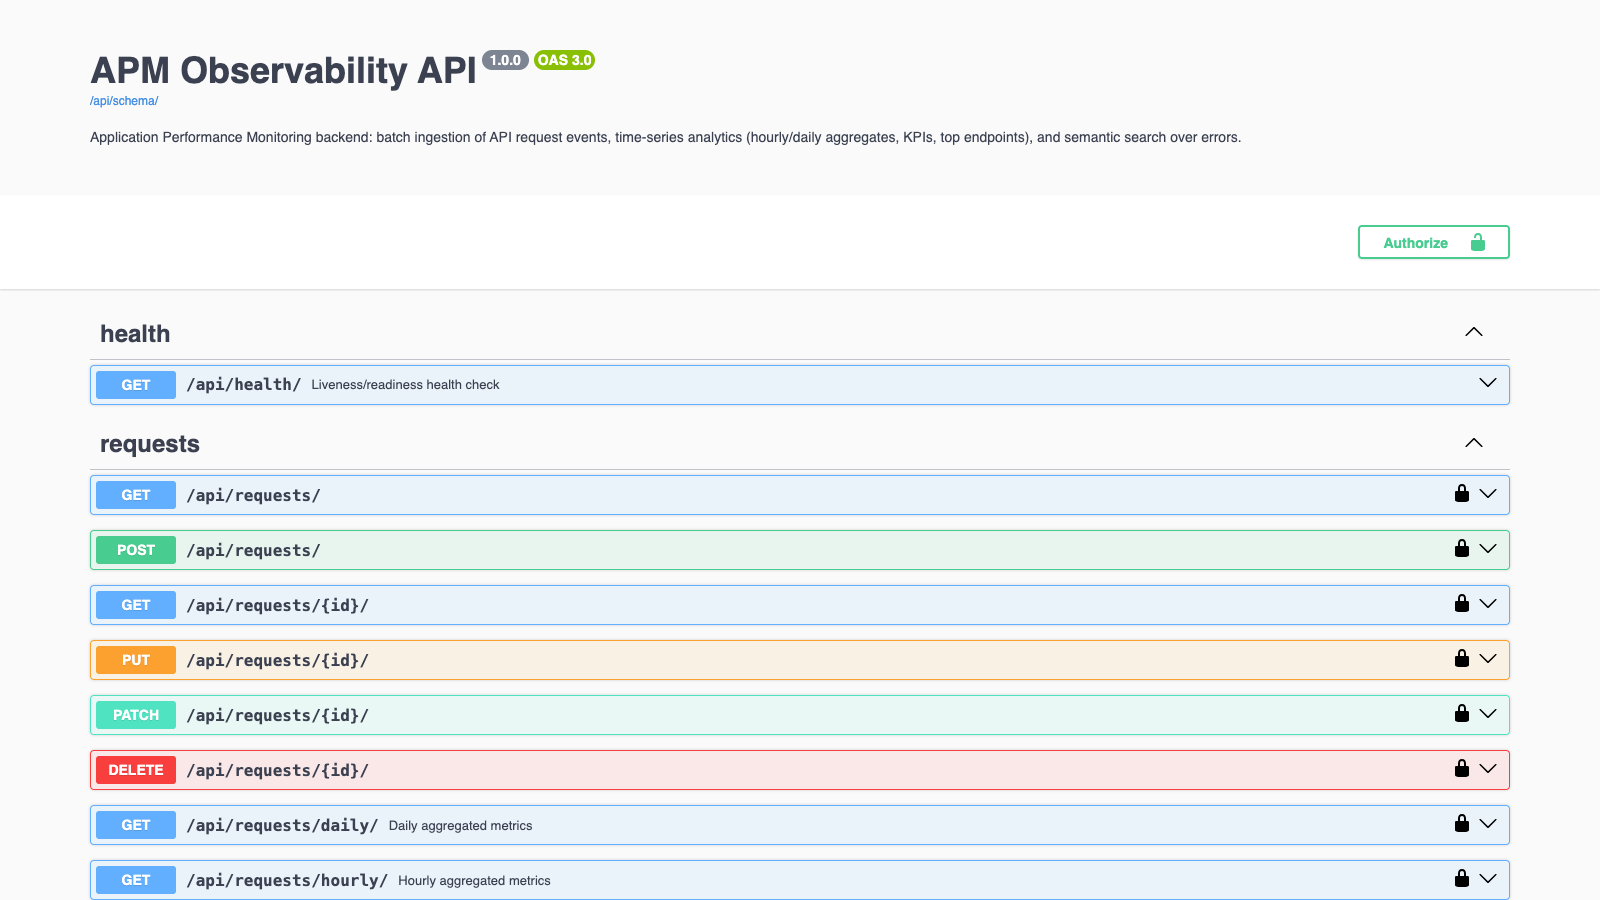
\includegraphics[width=0.9\textwidth]{swagger_ui.png}
    \caption{Documentation interactive de l'API (Swagger UI)}
    \label{fig:swagger-ui}
\end{figure}

\subsection{Tests de charge (k6)}
Une suite \texttt{k6} (\path{loadtest/ingest_and_read.js}) génère une montée en
charge progressive contre les endpoints d'ingestion et de lecture, en injectant
une proportion configurable d'événements en erreur (5xx) afin de faire réagir la
chaîne d'observabilité~\cite{k6-docs}. Des seuils (\emph{thresholds}) transforment
le test en garde-fou de performance.

\begin{verbatim}
make demo        # démarrer la stack
make loadtest    # BASE_URL / BATCH / ERROR_RATIO paramétrables
\end{verbatim}

\begin{figure}[H]
    \centering
    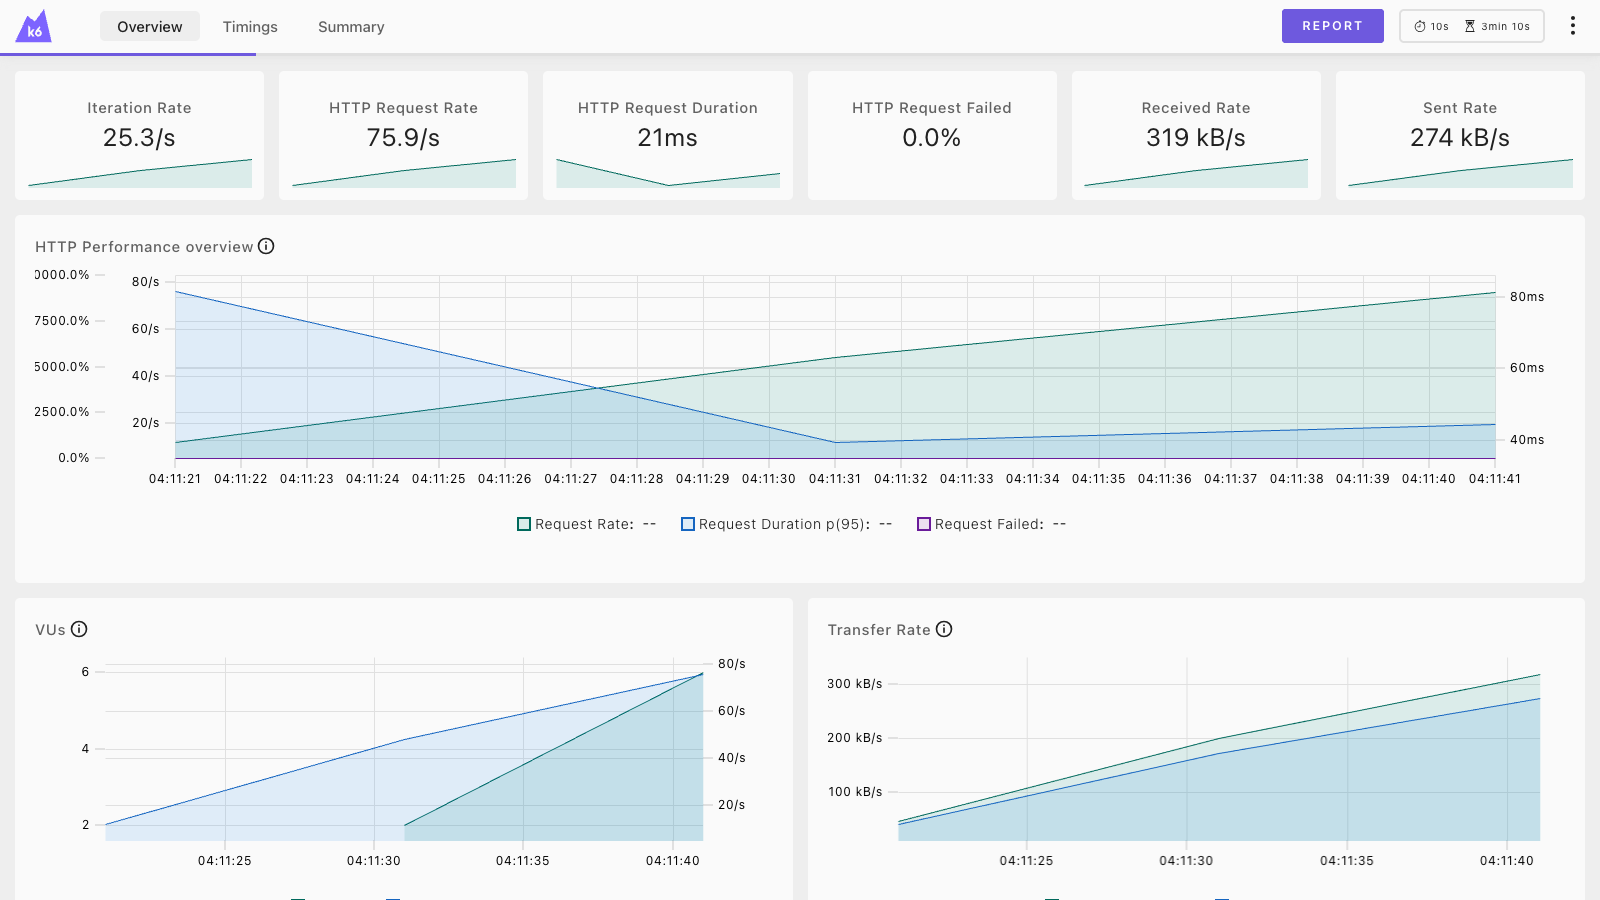
\includegraphics[width=0.9\textwidth]{k6_summary.png}
    \caption{Résultats du test de charge k6 (latence p95, taux d'erreur)}
    \label{fig:k6-summary}
\end{figure}

\subsection{Les trois piliers de l'observabilité}
La plateforme couvre désormais les trois piliers de l'observabilité, tous
consultables dans Grafana.

\subsubsection{Métriques}
Prometheus collecte les métriques applicatives (\texttt{django-prometheus} et des
métriques métier telles que \texttt{apm\_ingested\_requests\_total} et
\texttt{apm\_ingest\_latency\_seconds}), ainsi que \texttt{node-exporter} et
\texttt{postgres-exporter}.

\subsubsection{Traces distribuées (OpenTelemetry + Tempo)}
L'application Django est instrumentée avec OpenTelemetry ; les spans sont exportés
en OTLP vers un OpenTelemetry Collector qui les transmet à Grafana
Tempo~\cite{opentelemetry-docs,grafana-tempo}. Le traçage est activable via la
variable \texttt{OTEL\_ENABLED} et reste désactivé pendant les tests et
l'intégration continue.

\begin{figure}[H]
    \centering
    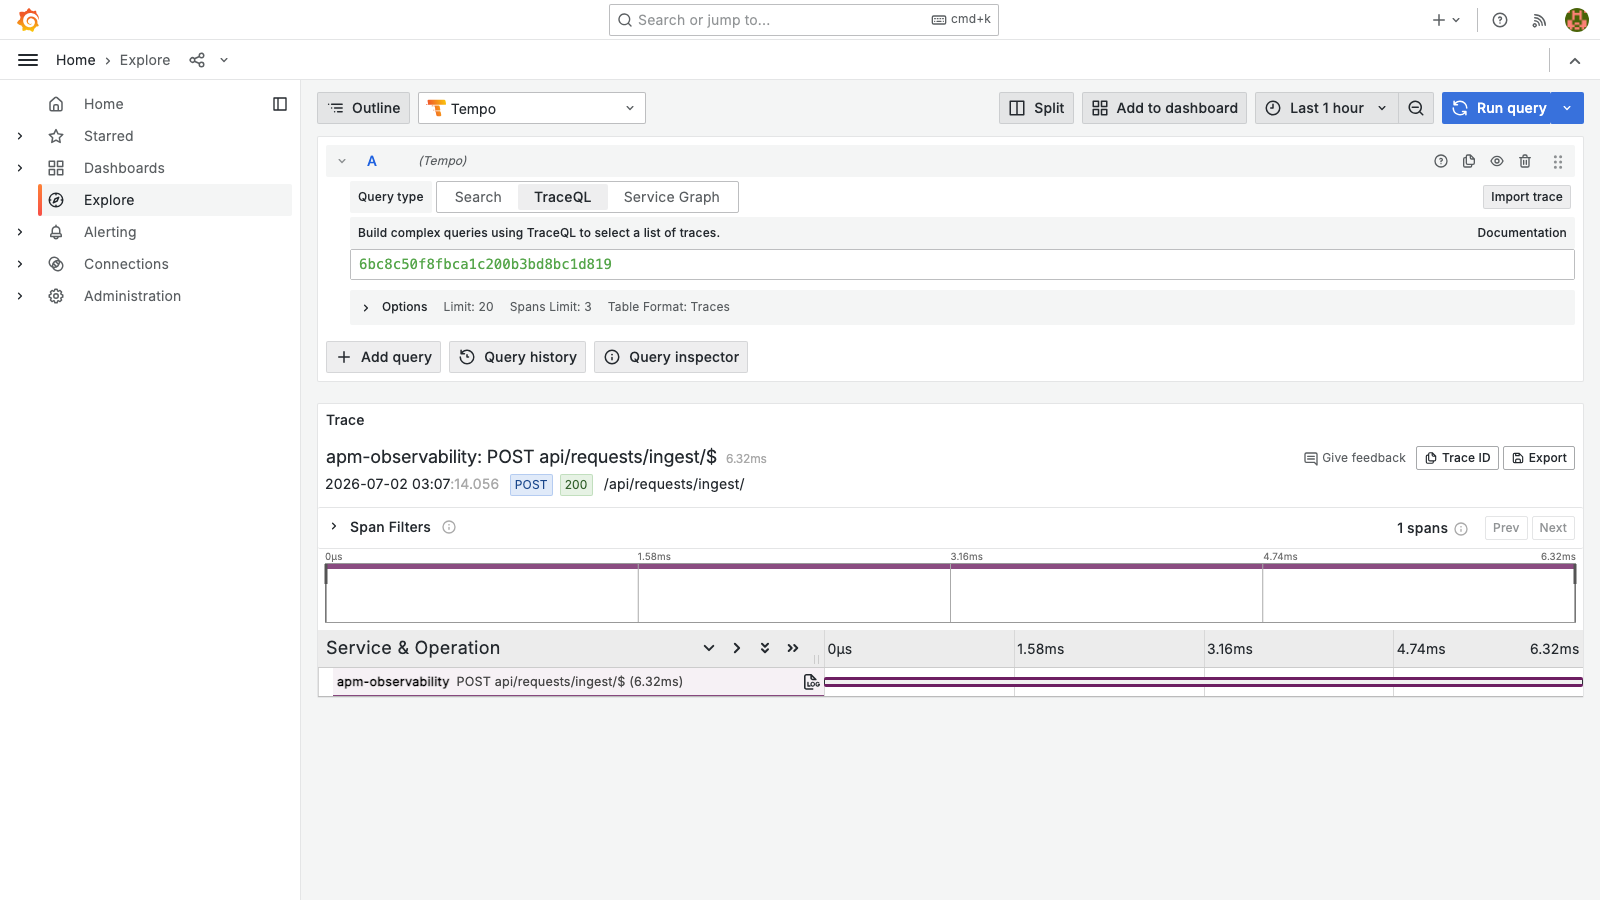
\includegraphics[width=0.9\textwidth]{tempo_trace.png}
    \caption{Trace distribuée d'une requête (Grafana Tempo)}
    \label{fig:tempo-trace}
\end{figure}

\subsubsection{Journaux structurés (Loki)}
L'application émet des journaux au format JSON incluant \texttt{trace\_id} et
\texttt{span\_id}. Promtail collecte les journaux des conteneurs et les expédie
vers Loki~\cite{grafana-loki}. Grafana relie les traces aux journaux (Tempo
$\rightarrow$ Loki) et inversement (Loki $\rightarrow$ Tempo).

\begin{figure}[H]
    \centering
    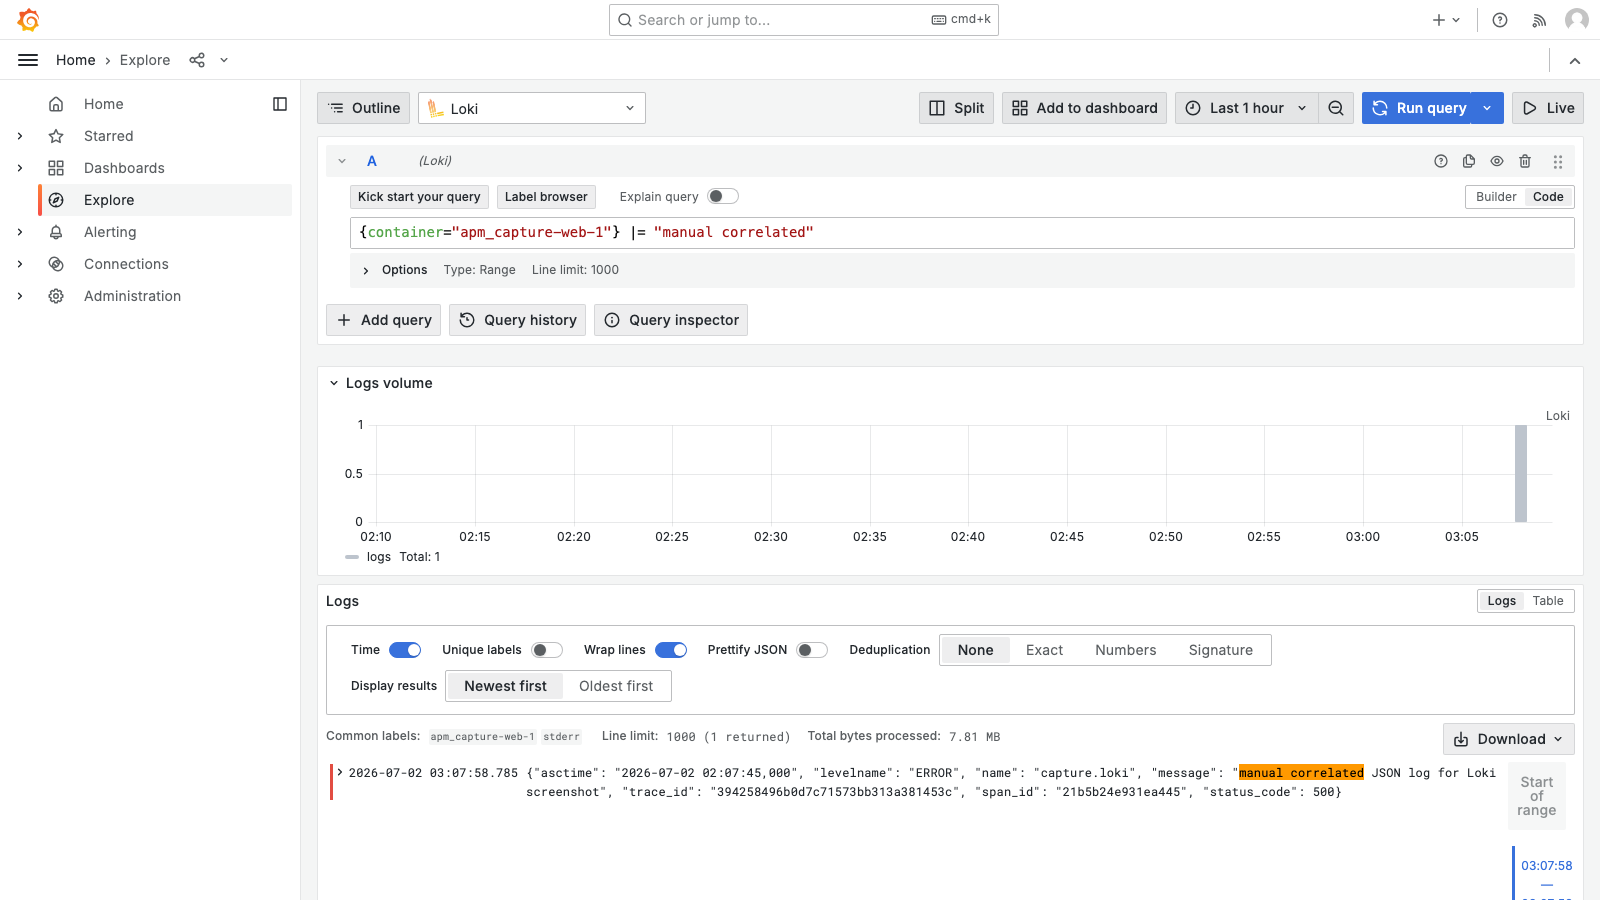
\includegraphics[width=0.9\textwidth]{loki_logs.png}
    \caption{Journaux structurés corrélés aux traces (Grafana Loki)}
    \label{fig:loki-logs}
\end{figure}

\subsection{Alerting orienté SLO}
Au-delà des alertes de seuil (taux d'erreur, latence, CPU), la plateforme définit
un objectif de niveau de service (SLO) de disponibilité à 99,5\,\% et des alertes
de consommation du budget d'erreur (\emph{burn-rate}) multi-fenêtres :
combustion rapide (14,4$\times$ sur 1\,h et 5\,min $\rightarrow$ alerte critique) et
combustion lente (6$\times$ sur 6\,h et 30\,min $\rightarrow$ avertissement), selon la
méthodologie du \emph{Google SRE Workbook}~\cite{google-sre-slo}.

\begin{figure}[H]
    \centering
    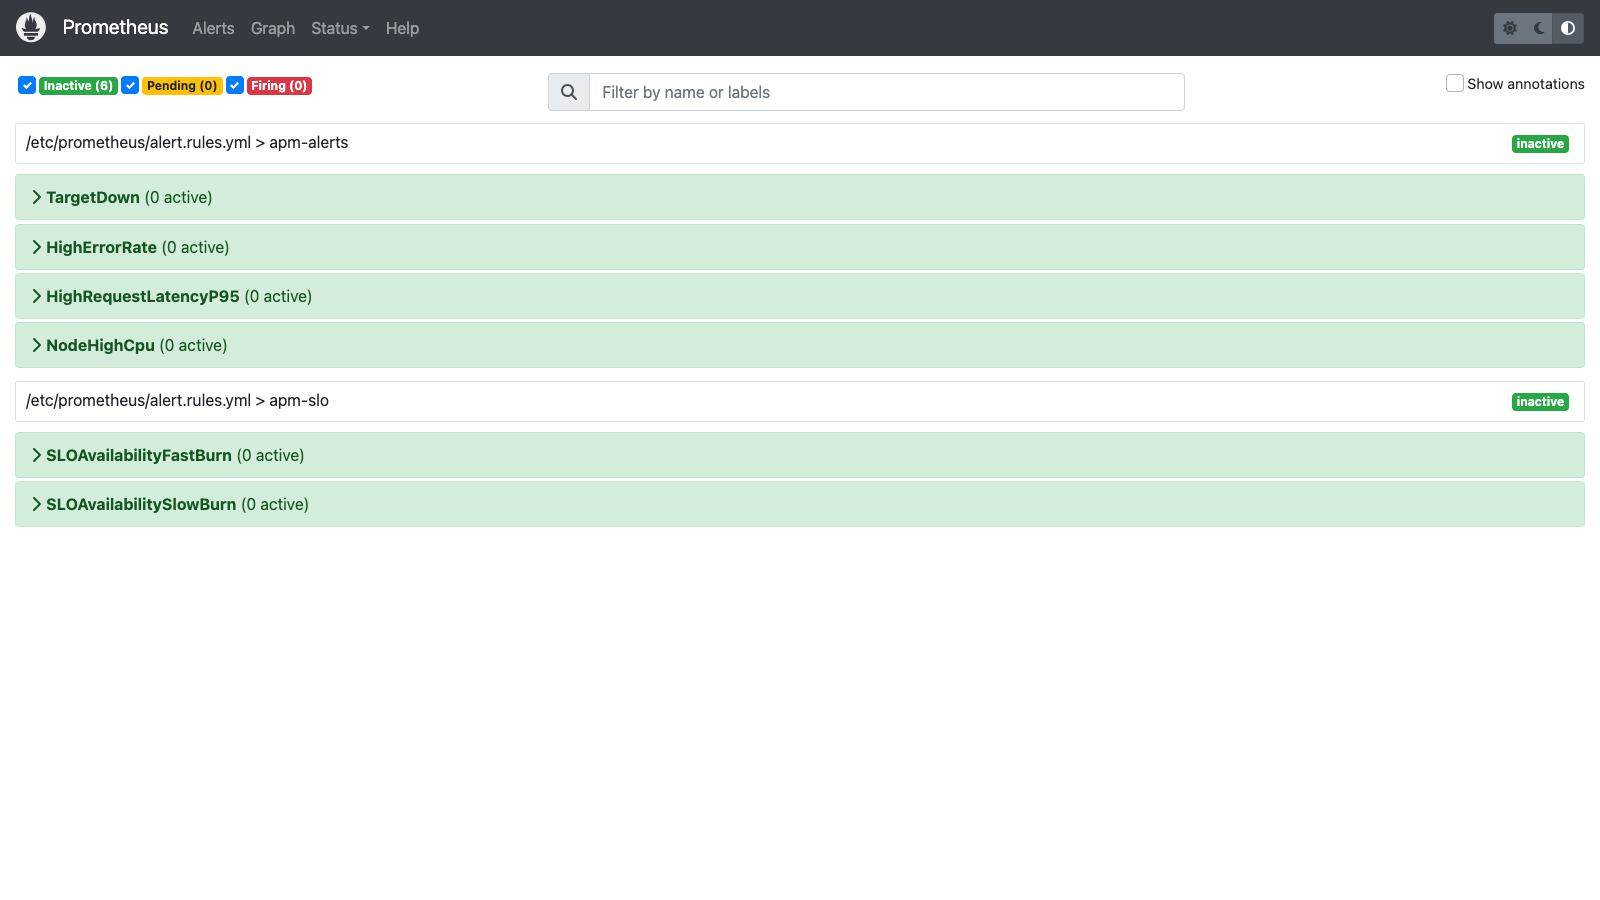
\includegraphics[width=0.9\textwidth]{prometheus_alerts.png}
    \caption{Alertes de budget d'erreur (Prometheus / Alertmanager)}
    \label{fig:prometheus-alerts}
\end{figure}

\subsection{Cycle de vie et qualité des données}
La migration \texttt{0009\_retention\_compression} active la compression
colonnaire native de TimescaleDB (par défaut au-delà de
\texttt{APM\_COMPRESS\_AFTER\_DAYS} = 7 jours) ainsi qu'une politique de rétention
(\texttt{APM\_RETENTION\_DAYS} = 90 jours) sur l'hypertable brute, les vues
continues conservant l'historique agrégé de long terme~\cite{timescaledb-compression}.

Une commande \texttt{check\_data\_quality} vérifie l'absence de valeurs manquantes,
la validité des plages (\texttt{status\_code}, \texttt{latency\_ms}), le taux de
\texttt{trace\_id} dupliqués et la fraîcheur des données. Elle renvoie un code de
sortie non nul en cas de violation, ce qui permet de l'utiliser comme garde-fou en
intégration continue.

\begin{verbatim}
python manage.py check_data_quality --max-age-minutes 60 --fail-on-empty
\end{verbatim}

\subsection{Chaîne CI/CD sécurisée}
Le pipeline d'intégration continue (lint, formatage, tests SQLite et TimescaleDB,
smoke Docker Compose, audit des dépendances) est complété par un garde-fou de
qualité des données et par des contrôles de sécurité : analyse statique CodeQL et
scan de vulnérabilités de l'image conteneur avec Trivy~\cite{trivy-docs}. La
livraison continue construit et pousse l'image vers GHCR avec génération d'un SBOM,
attestation de provenance et signature Cosign.

\subsection{Déploiement Kubernetes (Helm + GitOps)}
En complément de Docker Compose et d'Ansible, un chart Helm
(\path{deploy/helm/apm-observability}) décrit le déploiement de l'application sur
Kubernetes (Deployment, Service, Ingress, ConfigMap/Secret, HPA, et une
TimescaleDB en cluster optionnelle)~\cite{helm-docs}. Une \emph{Application} Argo CD
(\path{deploy/argocd/application.yaml}) assure une livraison déclarative en GitOps :
le cluster est maintenu en synchronisation avec le chart versionné dans Git, avec
auto-réparation et élagage des ressources~\cite{argocd-docs}.

\begin{verbatim}
helm lint deploy/helm/apm-observability
helm install apm deploy/helm/apm-observability --namespace apm --create-namespace
kubectl apply -f deploy/argocd/application.yaml   # variante GitOps
\end{verbatim}

\begin{figure}[H]
    \centering
    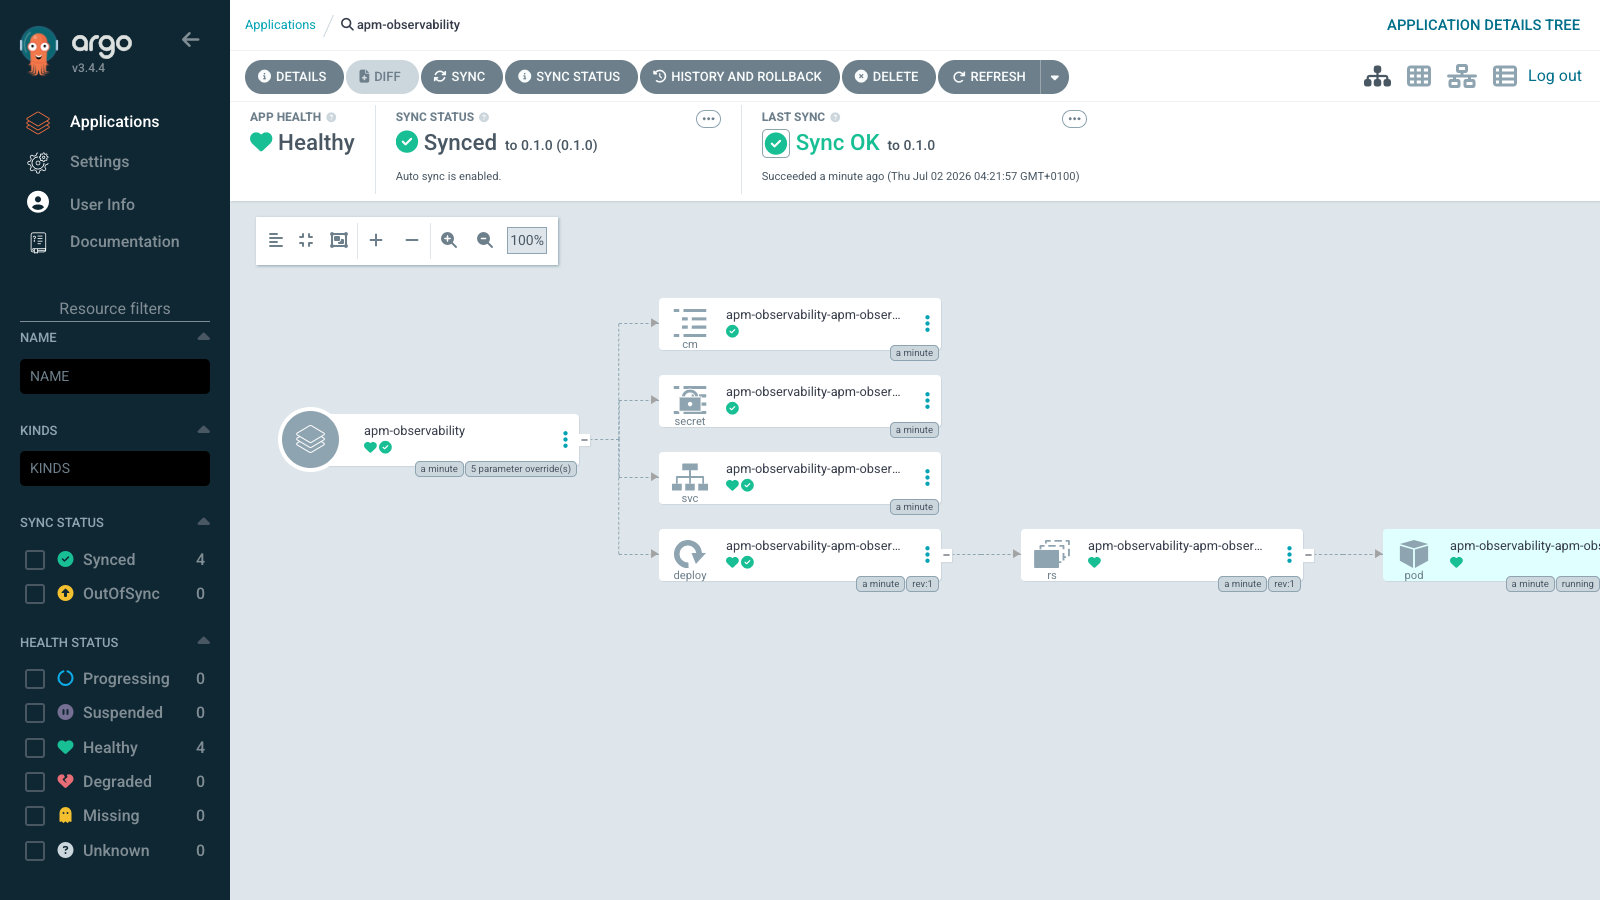
\includegraphics[width=0.9\textwidth]{argocd_app.png}
    \caption{Livraison GitOps de la plateforme (Argo CD)}
    \label{fig:argocd-app}
\end{figure}

\clearpage
\section{Conclusion et perspectives}

Ce travail a permis de mettre en place une plateforme d’observabilité APM cohérente, couvrant l’ingestion, le stockage, l’analyse et la visualisation des données. L’usage de TimescaleDB pour les séries temporelles, associé à des vues continues pour les KPI, apporte un socle performant et maintenable. La supervision couvre les trois piliers de l’observabilité --- métriques (Prometheus), journaux (Loki) et traces distribuées (OpenTelemetry + Tempo) --- consolidés dans Grafana, tandis que l’intégration des sauvegardes pgBackRest avec MinIO améliore la résilience globale. Les jeux de tests Postman/Newman et les scripts de déploiement documentés rendent la solution reproductible.

Sur le plan d’architecture, nous avons validé une configuration en mode cluster adaptée aux besoins de supervision et de charge. Ce choix facilite l’évolutivité, la séparation des responsabilités et la montée en puissance future. Dans un contexte de production, le cloud reste souvent le meilleur compromis en termes de coût, d’élasticité et d’exploitation, tandis que l’on-premise répond surtout aux exigences fortes de souveraineté et de conformité.

\subsection*{Apports d'industrialisation}
Au-delà du socle initial, la plateforme a été industrialisée sur plusieurs axes :
\begin{itemize}
    \item alerting orienté SLO avec règles de \emph{burn-rate} multi-fenêtres sur le budget d’erreur ;
    \item traçage distribué OpenTelemetry exporté vers Tempo, et journaux structurés corrélés dans Loki ;
    \item cycle de vie des données : compression et rétention TimescaleDB, plus un contrôle automatisé de la qualité des données ;
    \item documentation d’API auto-générée (OpenAPI / Swagger) et tests de charge k6 servant de garde-fou de performance ;
    \item chaîne CI/CD sécurisée : lint, tests, scan de vulnérabilités (Trivy), analyse statique (CodeQL), SBOM et signature d’image (Cosign) ;
    \item déploiement Kubernetes via un chart Helm et une livraison GitOps avec Argo CD.
\end{itemize}

\subsection*{Perspectives}
Plusieurs axes peuvent encore enrichir la plateforme :
\begin{itemize}
    \item échantillonnage et quotas de traces pour maîtriser le volume en forte charge ;
    \item autoscaling piloté par les métriques applicatives (par exemple via KEDA) ;
    \item externalisation des secrets (Vault, External Secrets) et rotation automatisée ;
    \item promotion multi-environnements en GitOps (dev / staging / prod) ;
    \item détection d’anomalies sur les séries temporelles et exploitation des \emph{embeddings} pgvector ;
    \item tests de résilience (chaos engineering) sur la bascule primaire/réplica et les pannes de stockage.
\end{itemize}

\clearpage
\appendix
\input{annexes}

\clearpage
\bibliographystyle{IEEEtran}
\bibliography{references}
\end{document}
